\shortpoint{ The paper is well organized into main sections of System Design,
	Dynamic Modeling, and a combined section of Experiments and Results. }
\shortreply{ We thank the reviewer for the good comment about the paper organization.}

\begin{point}
The details of the experiments performed with the controllers are
scarce, and should be elaborated for greater clarity. Phrases like "the
experimenter pushed the end-effector on the surface" leave the
direction of pushing unclear. Was there any instruction or consistency
in the forces applied (e.g., planar, orthogonal to the surface, etc.)?
\end{point}
\begin{reply}
	Based also on the comments received from all other reviewers, the experimental section has been completed revised. One of the experiments has been completely remade with 10 subjects and in two velocity conditions, figures have been changed.
	The test is now performed referring to similar tests performed in other paper such as  \cite{just2018exoskeleton}, and the description test has been significantly improved, adding also a picture of a user wearing the device during the test.
\end{reply}

\begin{point}
The text is mostly technically accurate with some usage of ambiguous
terms as mentioned above. However, it should be noted that there are 44
equations within the main paper and the Appendix, and these should be
reviewed carefully by the authors for accuracy. 
\end{point}
\begin{reply}
We have made  a strong effort to reduce the number of equations, so that now the overall explanation is more synthetic. The 3 control inputs have been described in terms of the same dynamic equations, as it should be, removing some not useful duplication of terms. Some of the equations have been formatted to outline the major contributions to the control. 
\end{reply}

\begin{point}
The clarity of text is a bit sporadic. It is clear and professional
throughout much if the writing. However, there are numerous
grammatically awkward phrases and some examples of unclear text needing
rewording for clarity. It is therefore recommended that the work be
proofread by a native English speaker.  Some examples are provided in the comments below.
\end{point}
\begin{reply}
We thanks the reviewers, the text was revised and proofread by a native English speaker, to improve correctness and overall flow.
\end{reply}
%
%\shortpoint{ Some examples are provided in the comments below. }
%\shortreply{ Fixed.}

\begin{point}
 Also, there are currently 22 individual figures.
Some of these would be better organized as subfigures together with
other closely-related images, diagrams, or illustrations, to lessen the
burden on the reader of drawing connections between aspects of the
work. Figures 6, 8, and 9, for example are highly related and it could
be argued that they could easily be merged into a single, more cohesive
figure. 
\end{point}
\begin{reply}
We thanks the reviewer for this wise comments. We spent a big effort in reorganizing all figures in view of simplifying the overall picture. The changes should be clearly visible between the two papers versions, as most figures were merged to present in a more synthetic way the results. 
\end{reply}

\begin{point}
Other sections could benefit from additional figures, such as
the experimental setup. There is not figure in the paper that shows the
device in use by a user to illustrate how the arm is configured
relative to the joints and end-effector. Some text seems to insinuate
that the hand holds the end-effector but the rest of the joints are not
aligned with the anatomical joints of the user. Images of the testing
setup would help alleviate such ambiguity.
\end{point}
\begin{reply}
We have now added figure 11 that shows the experimental set-up.

\begin{figure}[htb]
	\centering
	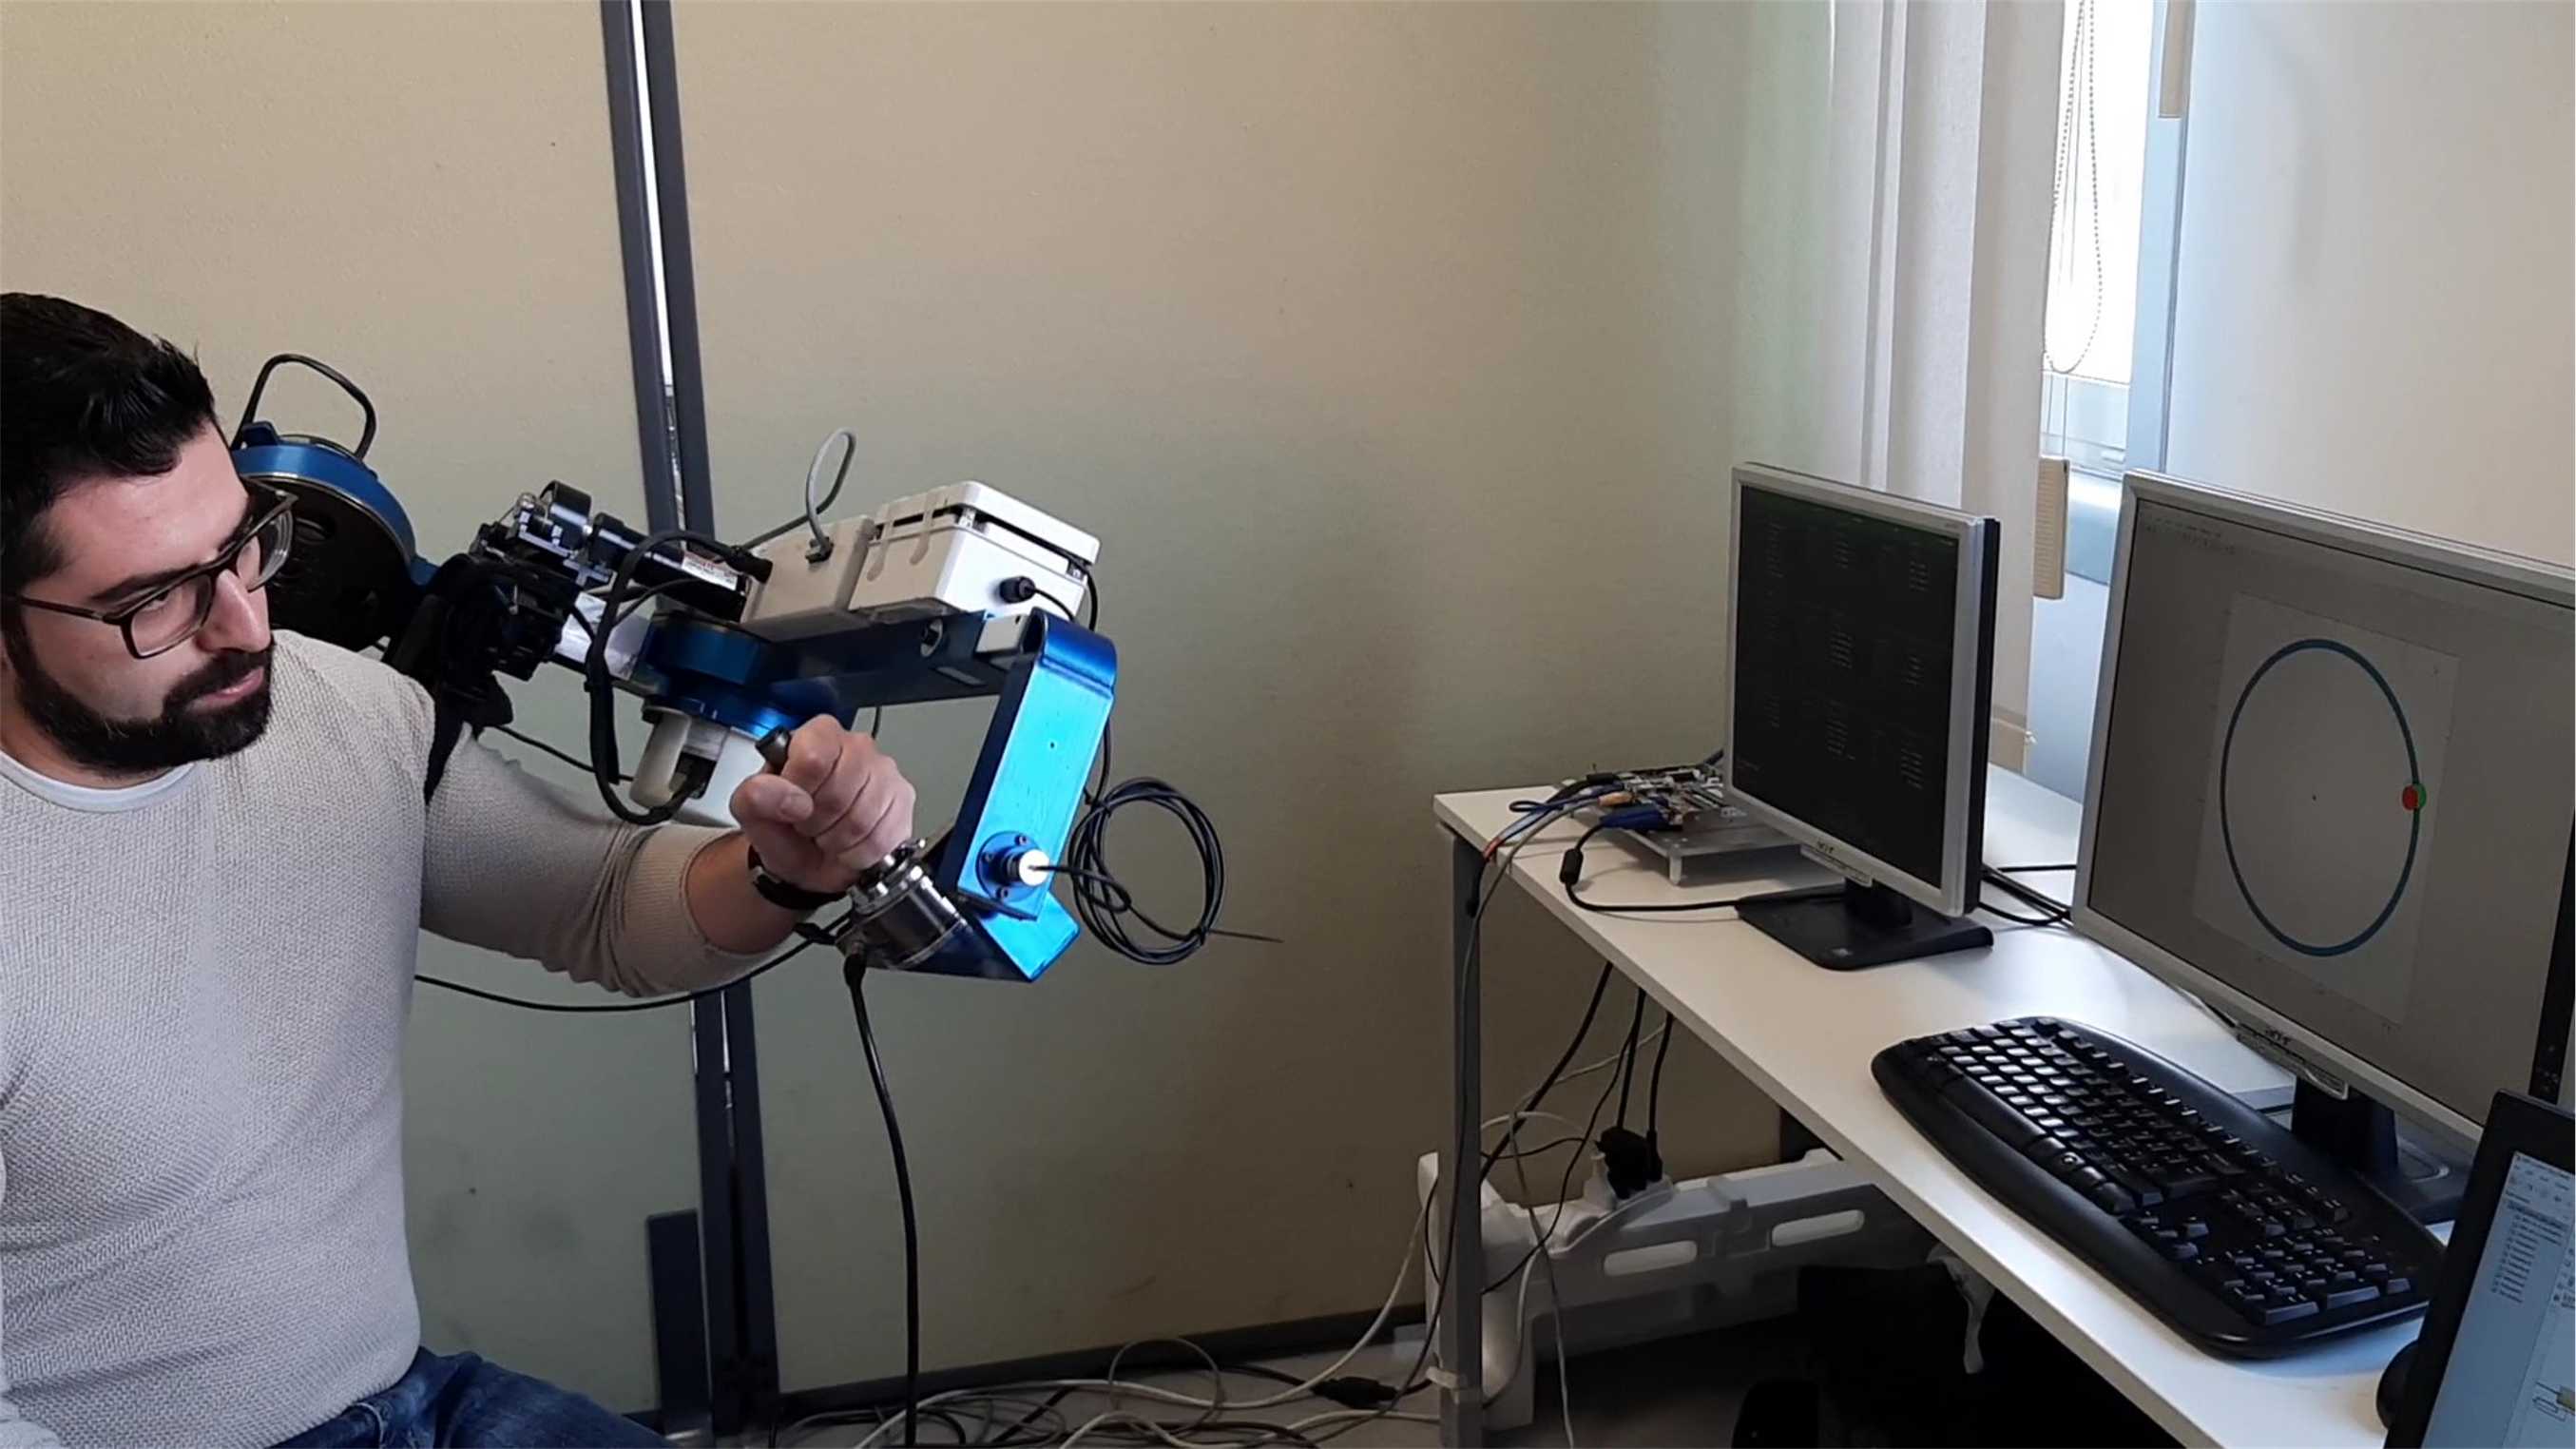
\includegraphics[width=0.5\columnwidth]{../imgRevised/experiment_setup}
	\caption{Experimental setup of the transparency test.}
	\label{fig:experimentalSetup}
\end{figure}

\end{reply}

\shortpoint{ Citations appear adequate. }
\shortreply{ We thank the reviewer for its positive comment, some more citations were added to take into account other reviewers' suggestions.}

\subsection*{Minor}

\shortpoint{ There are numerous grammatical inconsistencies involving the use of
	plurals and prepositions.}
\shortreply{ We thank the reviewer for its careful reading. We proofread the work several times in order to minimize the grammatical errors.}


\shortpoint{Abstract: "for several applications" seems vague and irrelevant in the
	opening sentence.}
\shortreply{ In view of the numerous comments, the abstract was rewritten and this sentence was completely revised.}


\shortpoint{Abstract: influence performances in term of $\rightarrow$ influence performance
	in terms o. Abstract: an other $\rightarrow$ [another]}
\shortreply{ The sentence was rewritten.}


\shortpoint{Abstract: complexity, maximum torque, transparency and haptic
	capabilities $\rightarrow$ complexity, maximum torque, transparency, and haptic
	capabilities
	This is a minor and common mistake, but lists of 3 or more things
	should have a comma also before the "and". Check paper throughout,
	including title. }
\shortreply{ The sentence was rewritten.}


\shortpoint{Some inconsistent formatting, missing plurals, missing oxford commas,
	and incorrect verb tenses (noted in pdf)}
\shortreply{ We thank the reviewer. We try to improve the grammar and fix errors.}
. 

\shortpoint{Some awkward formulation of infinitive verb forms: "allows to obtain"
	should be replaced by "allows it to obtain" or "allows obtaining".
	Check for similar throughout paper, e.g.: 
	capable to exert $\rightarrow$ capable of exerting 
	capable to infer $\rightarrow$ capable of inferring}
\shortreply{ We thank you particularly the reviewer for this suggestion, as this is a common error made by non-native English speaker in the improper usage of allow and capable. This has been fixed.}


\shortpoint{Page 2: awkward phrasing: "for what concern transparency" $-->$
	"regarding transparency"}
\shortreply{ Fixed.}


\shortpoint{Page 2: what does it mean to evaluate at geometrical level the
	quantitative and qualitative behavior of the controller? This portion
	of the introduction is important to provide the user with an
	understandable overview of what's to come. Further effort should be
	made to make the text more reader friendly and less ambiguous.}
\shortreply{ We agree with the reviewer that this sentence was unclear and has been reformulated as follows:
	{\em  As far as haptic rendering, the stability behavior and quality of force rendering of the proposed controller was assessed through a virtual wall simulation implemented with increasing  stiffness values and  compared it with the other two  benchmark controllers.}}


\shortpoint{Page 3: controls $\rightarrow$ "controllers" or "control schemes"}
\shortreply{ This typo has been fixed.}


\shortpoint{Page 3: it seems odd that the value of 3.7 is given for both weight and
	inertia after the reduction. Is this a typo?}
\shortreply{ The correct figure for motor inertia is 2.5. This was corrected in the text.}


\shortpoint{Page 4: why is R defined here in text when not used in the equations
	(1) and (2)?}
\shortreply{ The reviewer is correct, the definition has been removed.}


\shortpoint{Page 4: the strain gauges were placed at a distance of 3mm from the
	extremities. How was this location determined besides just not being in
	the middle and not beign too close to the end?}
\shortreply{ This was estimated by means of FEM and was chosen closer to the ends to maximize sensitivity, but avoiding border effects due to the fillet radius.}


\shortpoint{Fig.8: some small text and the arrow pointing to the location of the
	sensor is not clear. Location of probe is not visible at all in black
	and white.}
\shortreply{ The figure was made again to be more clear.}


\shortpoint{Page 5: avoid using "(n+1)-th" link. Referring to the n-th link is
	okay, but n+1 would be less ambiguous as "link n+1".}
\shortreply{ We agree, the suggested notation was adopted.}


\shortpoint{Page 5: deputed to estimate $\rightarrow$ employed to estimate?}
\shortreply{Thanks, fixed.}


\shortpoint{Figure 12: this is a figure for 3 different joints, but only one curve
	is shown. Do they all have the same curve? Is this just for the motor
	or does it involve the link inertias as the term "Joint" would imply?}
\shortreply{ This involve a single joint mounted on a testbed with a calibrated inertia link mounted on it. The phase diagram was added as well to this figure. An explanation was added in the figure caption as {\em joint sensor torque vs. motor torque command in standardized testbed conditions.}}, while in the text it is stated {\em Considering an average link inertia, it can be obtained the natural frequency for each joint elastic transmission. Results are shown in the}


\shortpoint{Figure 17: it's not clear from the figure if the observations made in
	text are accurate. Although the position and acceleration are similar,
	the plots in (a) and (b) have different scales on both x and y axes
	which could contribute in part to the lower interaction torques. When
	plots are compared, their axes should be scaled equally.}
\shortreply{ Thanks, we agree, the corresponding figures has been now changed. The reviewer will find the new data in figure 14 and 15, where these observations were taken duly into account.}


\shortpoint{Figure 18: it would be nice to see the target circle, perhaps overlaid
	in white, on the plot for reference.}
\shortreply{ This figure was made again, now in figure 12 the suggestion of the reviewer was taken into account.}


\shortpoint{Page 12: few details are provided about the controller evaluation
	trials T1-T4 and the details provided use some ambiguous terms that
	don't help to clarify what was done. Please revise and add text to
	improve the clarity. }
\shortreply{ Fixed.}


\begin{point}
For additional markup and suggested revisions, see attached pdf.
\end{point}
\begin{reply}
The comments in the pdf were also implemented in the revised text. We take the occasion to thank the reviewer for the in-deep revision of the text.
\end{reply}